\chapter{Result}
\thispagestyle{empty}
In this chapter, result of this project is presented by using one package from ADL. In this way, this system can take advantage of existing SCORM 
compliant packages. The user interface for such functionality is shown below.
\begin{figure}[hb]
	\begin{center}
		\includegraphics[scale=0.3]{importing.png}
	\end{center}
	\caption{Importing User Interface.}
	\label{fig:importing}
\end{figure}
\section{Import whole package}
Manifest Basics Content Example Content Package \cite{mbce_package} is used. Figure~\ref{fig:importing} illustrates the interface for importing. The 
check box ``UploadSCORMZipFile'' is used to indicate whether user wants to upload SCORM zip file or just XML file. After importing, one folder was 
created for this package. The name of this folder is one GUID, which can prevent guessing and name-conflict. 
Figure~\ref{fig:result_import_whole_package} shows the content of this new created folder, which coincides with the content of this zip file. In 
other words, if the package is unzipped, the content is exactly the same to what is contained in this folder.
\begin{figure}[h]
	\begin{center}
		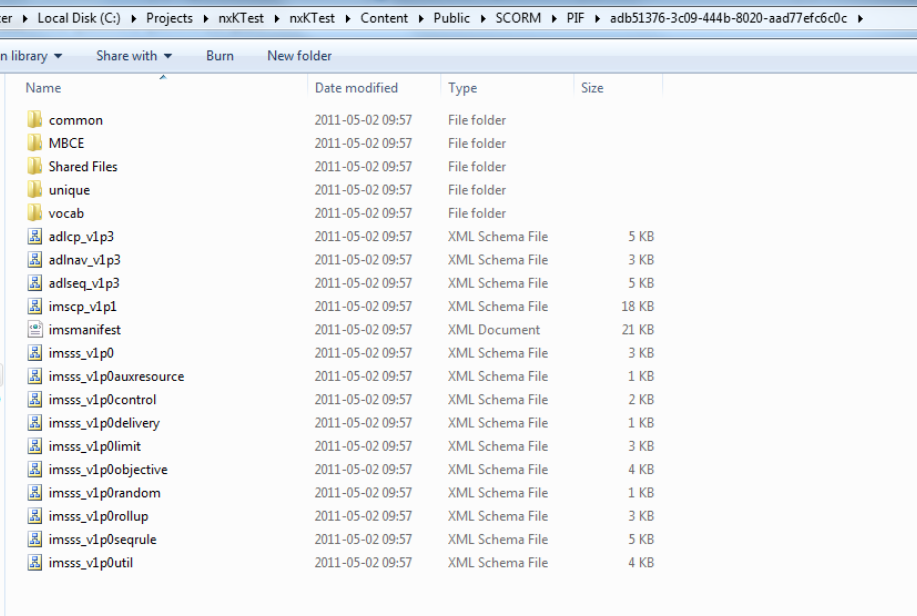
\includegraphics[scale=0.3]{result_import_whole_package.png}
	\end{center}
	\caption{Result of importing whole package.}
	\label{fig:result_import_whole_package}
\end{figure}
\begin{figure}[h]
	\begin{center}
		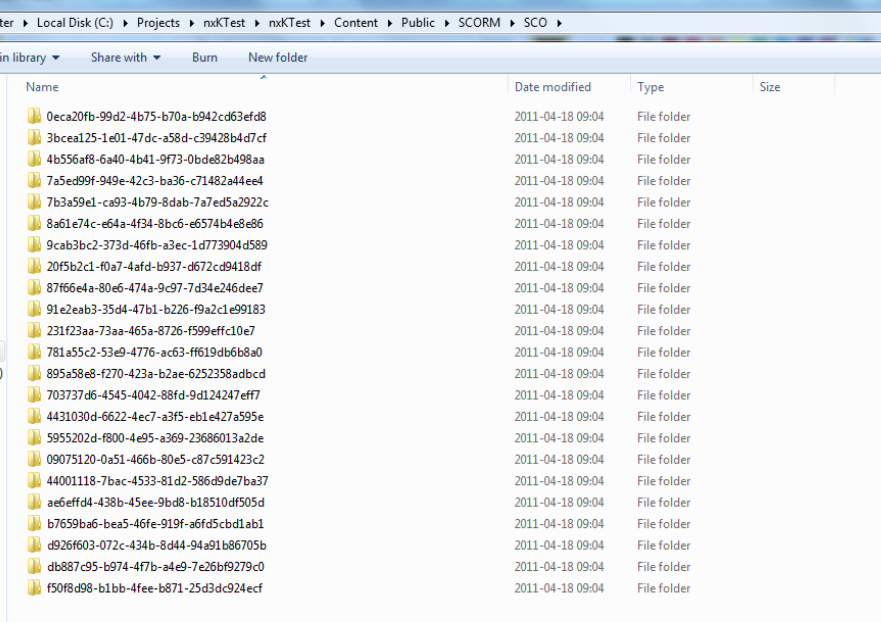
\includegraphics[scale=0.3]{result_import_single_scos.png}
	\end{center}
	\caption{Result of importing single SCOs.}
	\label{fig:result_import_single_scos}
\end{figure}
\begin{figure}[b]
	\begin{center}
		\includegraphics[scale=0.3]{result_presentation_sco.png}
	\end{center}
	\caption{Presentation of single SCO.}
	\label{fig:result_presentation_sco}
\end{figure}
\section{Import single SCOs}
Manifest Basics Content Example Content Package \cite{mbce_package} is used. The user interface is the same. The way to distinguish the two different 
importing(whole package or single SCO) has not implemented on the interface. It could be implemented as one check box. However, after consulting the 
company, I decided to hardcode the if condition, since someone in the company is particularly responsible for the user interface designing. In other 
words, the expression to evaluate within ``if'' is always true if I want to import the whole package, or always false if I want to import the SCOs.
After importing, a few folders are created for this package. They have one-to-one map to the SCOs in this package. 
Figure~\ref{fig:result_import_single_scos} shows all the new created folders.
\section{Presentation of SCO}
The ``Introduction to Manifests'' SCO in Manifest Basics Content Example Content Package \cite{mbce_package} is used, which is one very simple SCO, 
for it contains only one HTML page. Usually, one SCO will contain more than one HTML pages, then the SCO is responsible for the internal navigation. 
While navigating from one HTML page to another, the SCO might communicate with the LMS, which requires the LMS to implement all the APIs.
Figure~\ref{fig:result_presentation_sco} presents the content of this SCO.
